\chapter{Signal Extraction}
There are several significant SM processes that contribute to the background to the DM signal. 
The largest background process is events where a lepton is not properly reconstructed by the detector, resulting in a final state that passes the lepton vetoes. Background events of this nature are most likely to produce just a single lepton as well as \ptmiss from a neutrino and have several jets, such as semileptonic t$\bar{\mathrm{t}}$ events and W bosons produced in association with initial state jets. Examples of such processes can be seen in \cref{fig:w+jets,fig:ttbar}.  
The second largest background process is events where a Z boson is produced in association with jets. The Z then decays into two neutrinos, which has a branching ratio of roughly $\text{BR(Z}\to\nu\nu) = 0.2$~\cite{Zyla:2020zbs}. The presence of the neutrinos gives the event high \ptmiss, while the initial-state jets can pass the various cuts based on jet kinematics. A representative Feynman diagram of this process is shown in \cref{fig:z+jets}.
The next largest background process is multijet production.
The smallest relevant background are other processes where a Higgs boson is produced, such as the Zh and Wh processes.

\begin{figure}[ht]
\centering
     \begin{subfigure}[b]{0.25\textwidth}
         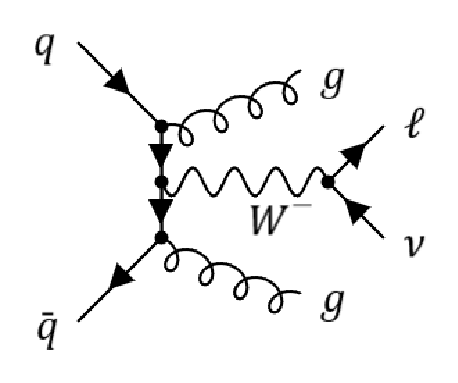
\includegraphics[width=\textwidth]{Chapters/Signal_Extraction/w+jets.pdf}
         \caption{A W boson decaying to a neutrino and a lepton in association with two partons.}
         \label{fig:w+jets}
     \end{subfigure}
     \begin{subfigure}[b]{0.25\textwidth}
         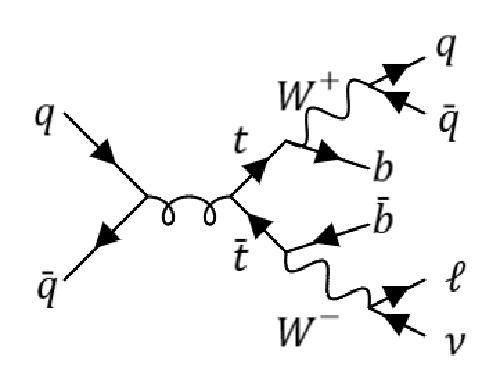
\includegraphics[width=\textwidth]{Chapters/Signal_Extraction/ttbar.pdf}
         \caption{\raggedright A t$\bar{\mathrm{t}}$ process where one W boson decays leptonically and the other decays hadronically.}
         \label{fig:ttbar}
     \end{subfigure}
    \begin{subfigure}[b]{0.25\textwidth}
         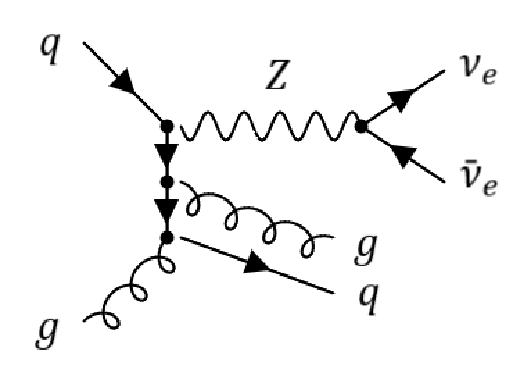
\includegraphics[width=\textwidth]{Chapters/Signal_Extraction/z+jets.pdf}
         \caption{A Z boson decaying to two neutrinos in association with two partons.}
         \label{fig:z+jets}
     \end{subfigure}
\caption{Feynman diagrams representing several processes that can contribute to the background of a 2HDM+a signal.}
\end{figure}

To estimate the level of background events in the final selection, it is useful to identify properties that are significantly different between the background and signal events. One useful variable for doing so is the mass of the highest-momentum AK8 jet in the event, referred to as $m_{\text{AK8}}$. 
Events resulting from multijet processes and Z or W boson production in association with initial state jets are expected to have low-mass jets, as most of these jets come from high-momentum gluons. 
However, in events where the decay of a heavy object such as a W boson or top quark is reconstructed as an AK8 jet, that jet will have a mass around $\GeV{80}$ and $\GeV{170}$, respectively. 
Finally, events from the signal or from the Higgs background processes will have an AK8 jet with a mass around that of the SM Higgs, $\GeV{125}$. These relative populations can be seen in \cref{fig:ak8massshape}. 
This suggests dividing events into 4 $m_\text{AK8}$ bins: $0\text{--}\GeV{50}$, $50\text{--}\GeV{100}$, $100\text{--}\GeV{150}$, and $>\GeV{150}$. Although the background estimations in this analysis are done using simulated events, adding mass sidebands allows these estimates to be constrained using a data-driven background estimation for an analysis done at the HL-LHC.

\begin{figure}[ht]
\centering
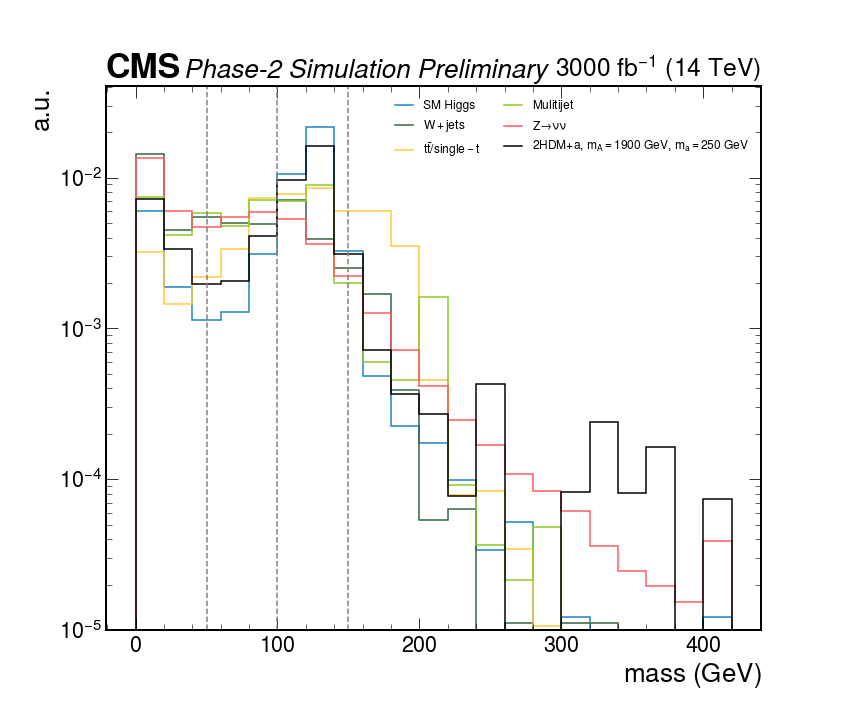
\includegraphics[width=0.845\textwidth]{Chapters/Signal_Extraction/shape_AK8_sdmass.png}
\caption{The $m_\text{AK8}$ distribution in the final selection. Shown here are the main backgrounds and the $m_\mathrm{A} = \GeV{1900}$, $m_\mathrm{a} = \GeV{250}$ signal. The histograms are normalized to an integral of 1.}
\label{fig:ak8massshape}
\end{figure}

In addition to $m_\text{AK8}$, there is a significant difference between the signal and background in the distribution of the minimum \mt of the AK8 jet-\ptmiss system, as can be seen in \cref{fig:mtshape}. The signal has a much more prominent tail, while the background peaks far earlier. 10 even \mt bins are selected between $600$ and $\GeV{2400}$ , with the last bin containing all events with \mt greater than $\GeV{2400}$. Multiple \mt bins are chosen in order to cover the wide range of masses of the pseudoscalar A that I examine in this thesis.

\begin{figure}[ht]
    \centering
    \begin{subfigure}[b]{\textwidth}
        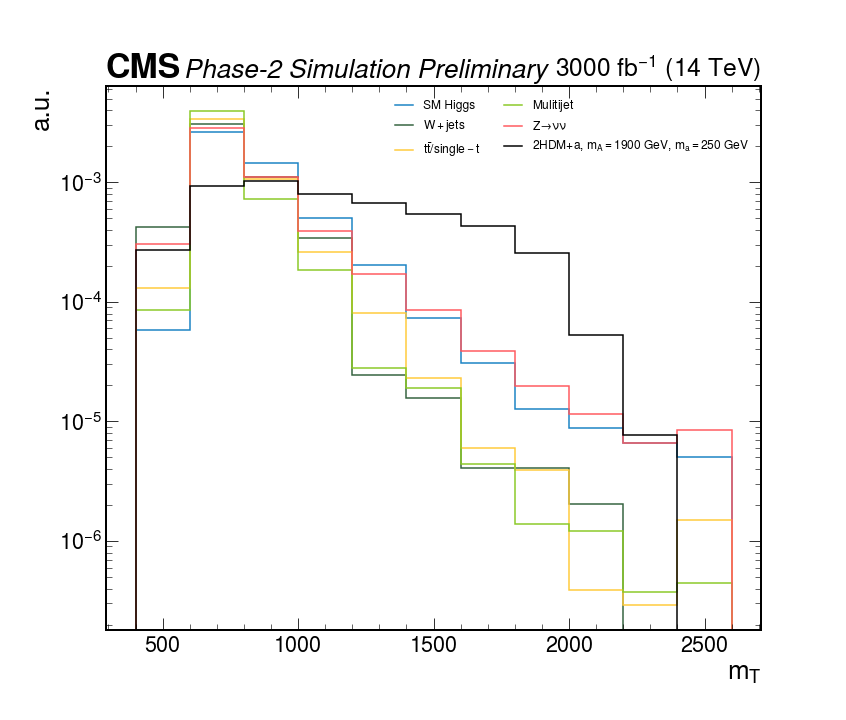
\includegraphics[width=0.845\textwidth]{Chapters/Signal_Extraction/shape_MT_backgrounds.png}
    \end{subfigure}
    \begin{subfigure}[b]{\textwidth}
        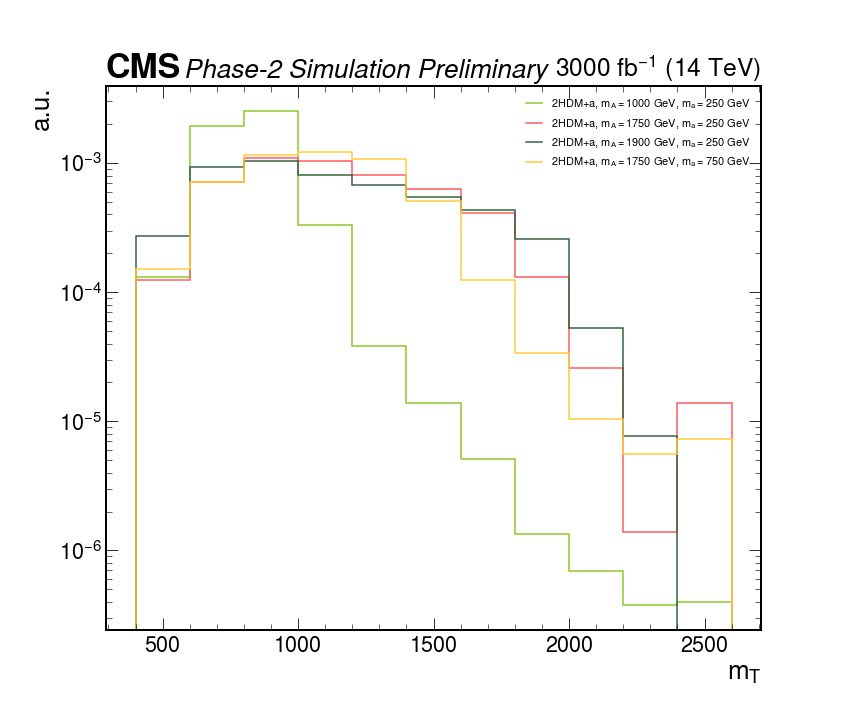
\includegraphics[width=0.845\textwidth]{Chapters/Signal_Extraction/shape_MT_signals.png}
    \end{subfigure}
\caption{The \mt distribution in the final selection. Shown in the upper plot are the main backgrounds against the $m_\mathrm{A} = \GeV{1900}$, $m_\mathrm{a} = \GeV{250}$  signal. The lower plot compares the $m_\mathrm{A} =1000$, $1750$, $\GeV{1900}$, $m_\mathrm{a} = \GeV{250}$ and $m_\mathrm{A} = \GeV{1750}$, $m_\mathrm{a} = \GeV{750}$ signals. The histograms are normalized to an integral of 1.}
\label{fig:mtshape}
\end{figure}

A histogram of the yields of the main backgrounds and two representative signal points is given in \cref{fig:srbins} showing the contribution of the signal and backgrounds in each bin, as well as the size of the post-fit uncertainties in each bin.

\begin{figure}[ht]
    \centering
    \begin{subfigure}[b]{\textwidth}
        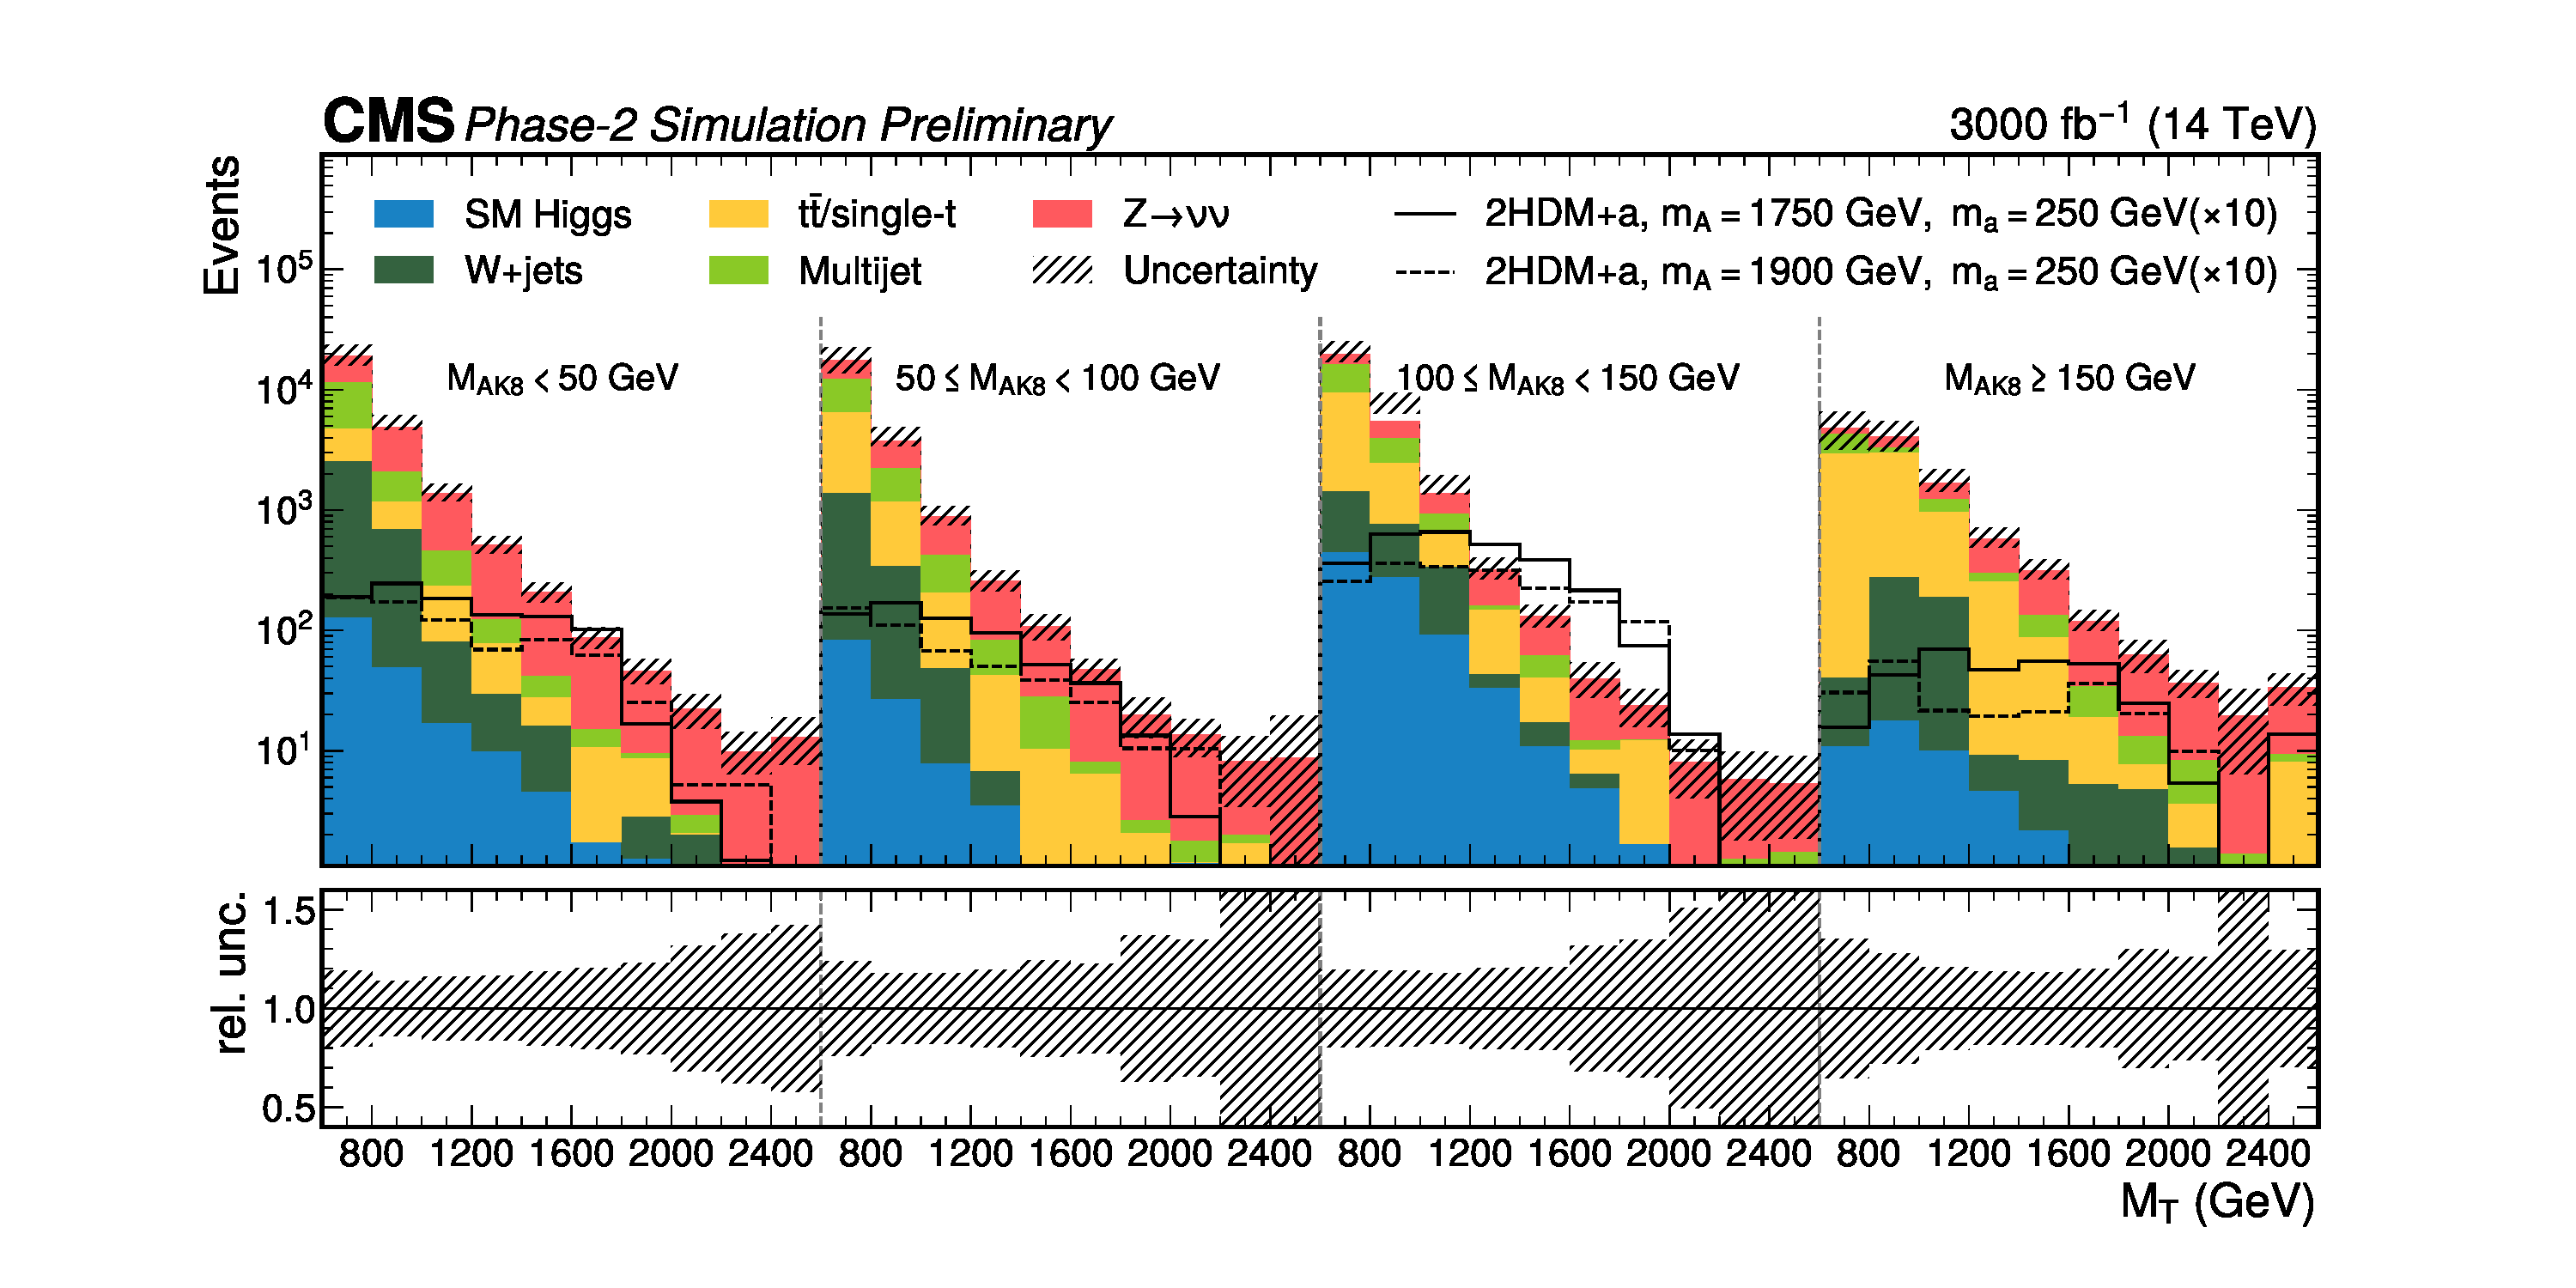
\includegraphics[width=\textwidth]{Chapters/Signal_Extraction/prefit_sr.pdf}
    \end{subfigure}
    \begin{subfigure}[b]{\textwidth}
        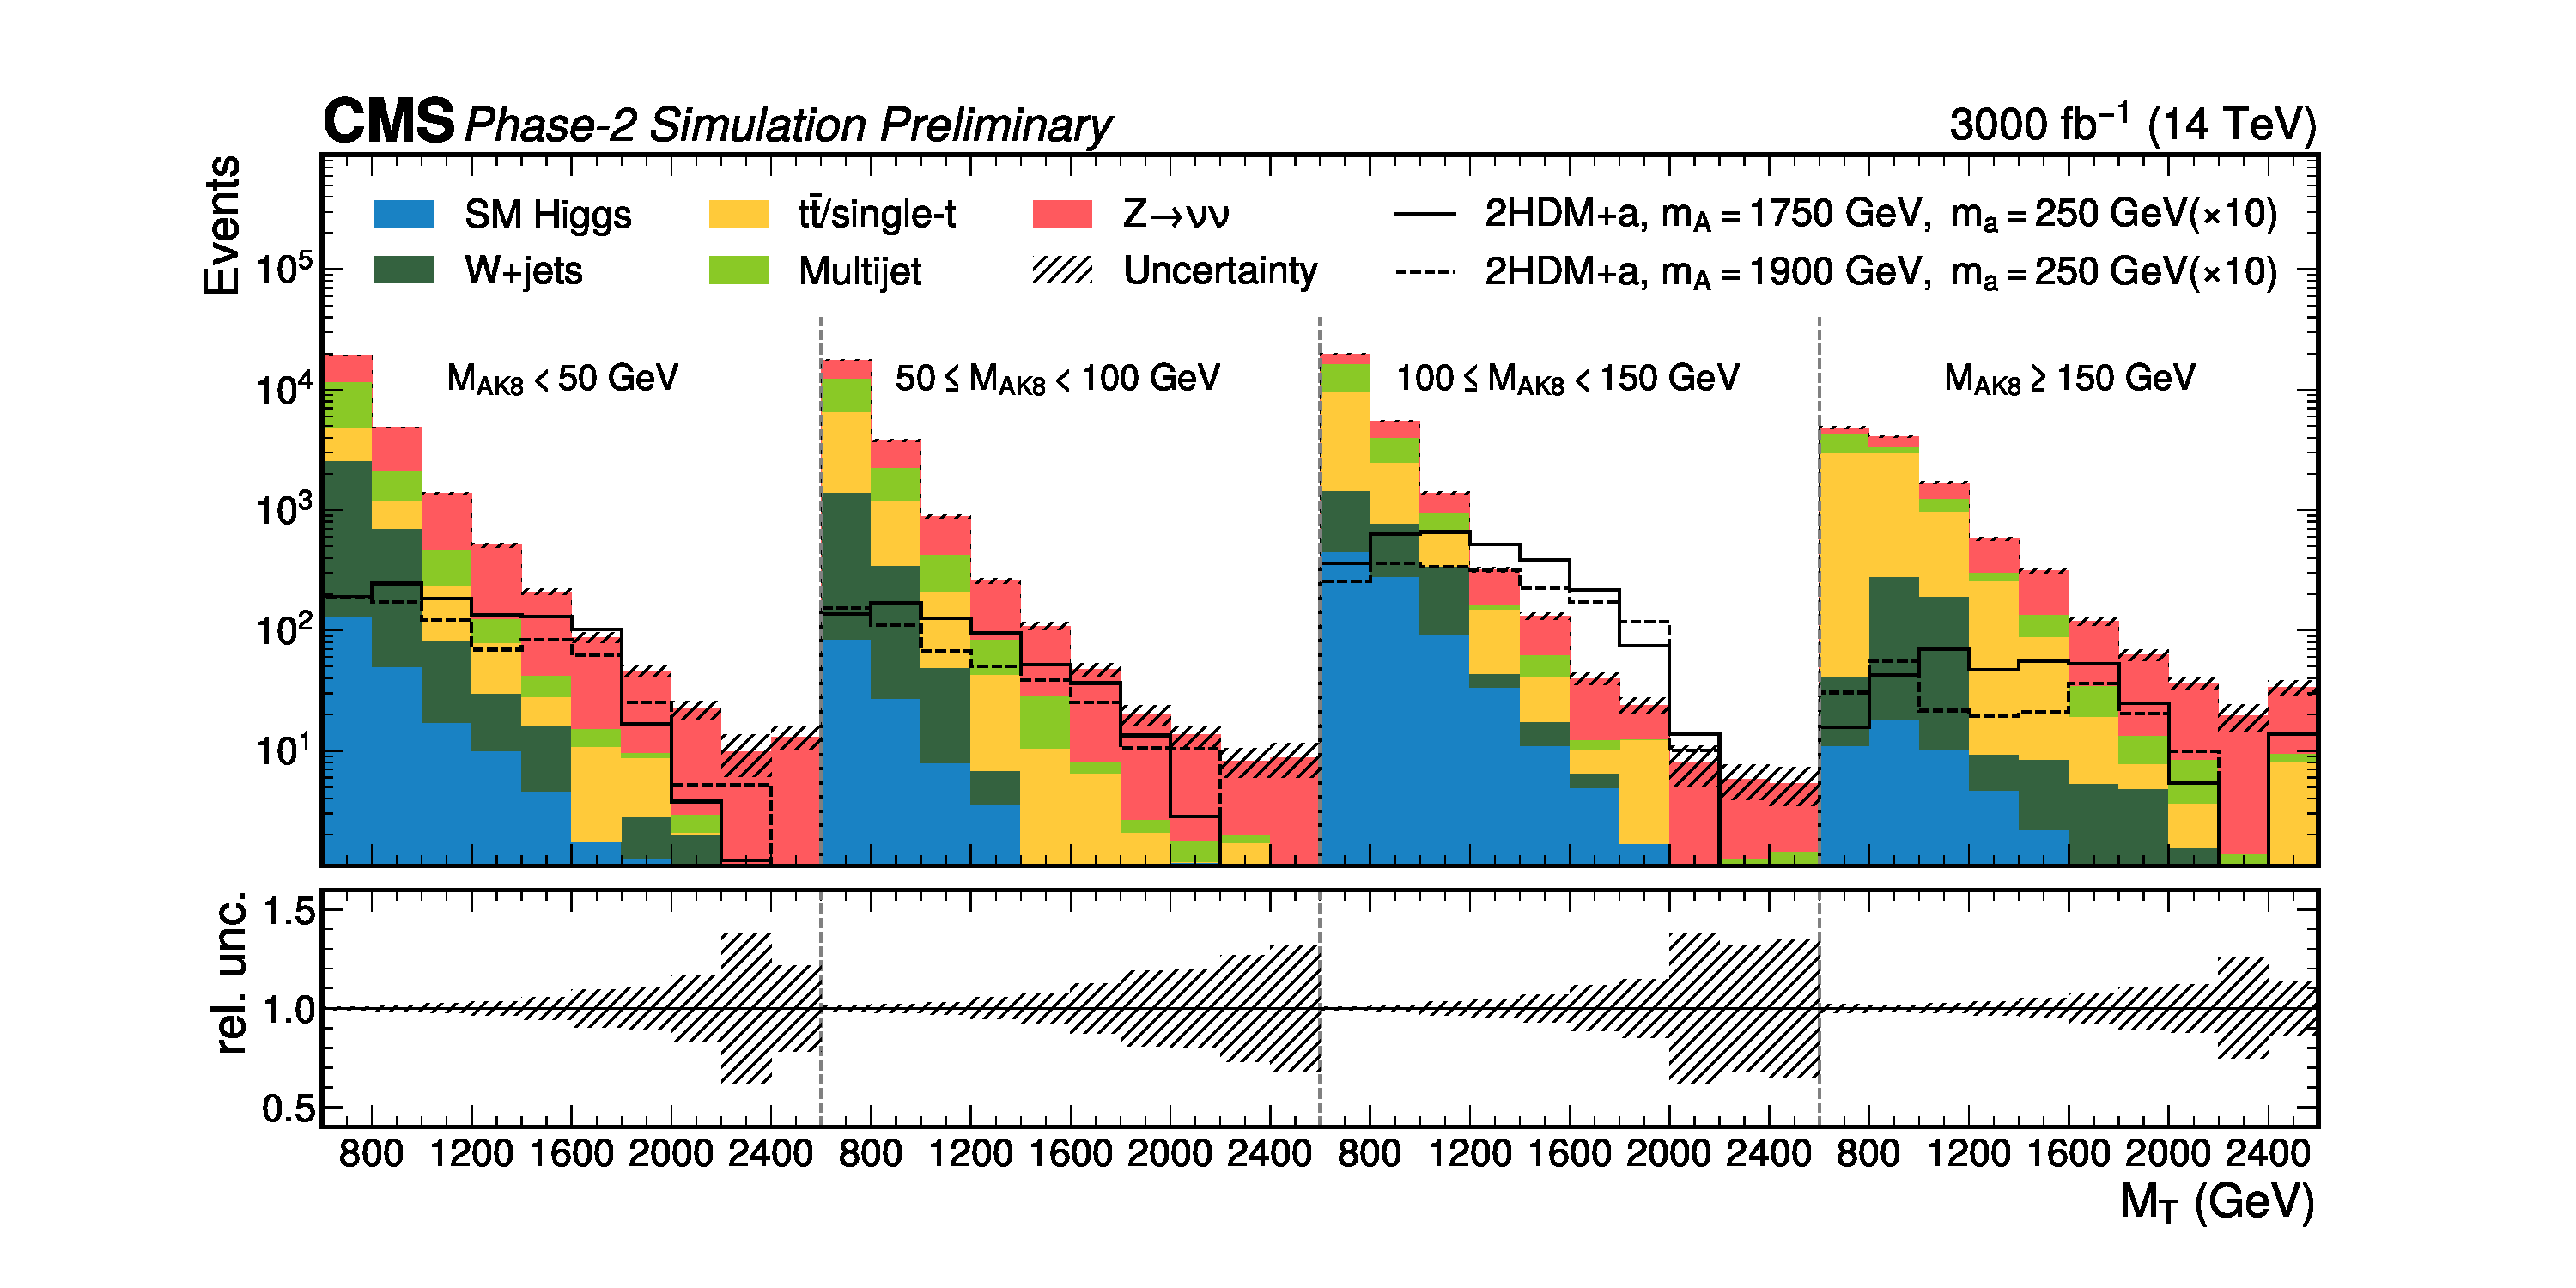
\includegraphics[width=\textwidth]{Chapters/Signal_Extraction/postfit_sr.pdf}
    \end{subfigure}
    \caption{The yield of the main backgrounds and two 2HDM+a signals with $m_\mathrm{A} = \GeV{1750}$, $m_\mathrm{a} = 250$, $\GeV{750}$. The signal is scaled tenfold for the purpose of contrasting the shape with the backgrounds. The total pre- and post-fit uncertainties in each bin are given by the shading, with the lower plot showing the relative uncertainty.}
    \label{fig:srbins}
\end{figure}